
\documentclass[12pt,a4paper]{article}
\usepackage[utf8]{inputenc}
\usepackage[T2A]{fontenc}
\usepackage[ukrainian]{babel}
\usepackage{amsmath}
\usepackage{graphicx}
\usepackage{booktabs}
\usepackage{float}
\usepackage{geometry}
\usepackage{colortbl}
\usepackage{xcolor}
\usepackage{fancyhdr}
\usepackage{titlesec}
\usepackage{array}
\usepackage{longtable}
\usepackage{siunitx}

\geometry{left=2.5cm,right=2.5cm,top=2.5cm,bottom=2.5cm}

\titleformat{\section}{\Large\bfseries}{\thesection}{1em}{}
\titleformat{\subsection}{\large\bfseries}{\thesubsection}{1em}{}

\pagestyle{fancy}
\fancyhf{}
\fancyhead[C]{\textbf{Звіт багатофакторної лінійної регресії}}
\fancyfoot[C]{\thepage}
\renewcommand{\headrulewidth}{0.4pt}

\begin{document}

\begin{center}
\Large\textbf{Звіт багатофакторної лінійної регресії}
\end{center}

\vspace{1cm}

\textbf{Дата:} \today

\vspace{0.5cm}

\section{Опис моделі}

\begin{itemize}
    \item Залежна змінна: \textbf{Sleep Hours}
    \item Незалежні змінні: \textbf{Sample Question Papers Practiced}
    \item Коефіцієнт детермінації $R^2$: \textbf{0.0000}
    \item Середньоквадратична похибка: \textbf{2.8756}
\end{itemize}

\vspace{0.5cm}

\section{Коефіцієнти регресії}

\begin{center}
\begin{tabular}{lcccc}
\toprule
\textbf{Змінна} & \textbf{Коефіцієнт} & \textbf{P-значення} & \textbf{Значущість (p < 0.05)} \\
\midrule
Вільний член & 6.5198 & Н/Д & Н/Д \\
Sample Question Papers Practiced & 0.0024 & 0.6899 & Ні \\

\bottomrule
\end{tabular}
\end{center}

\vspace{1cm}

\begin{figure}[H]
    \centering
    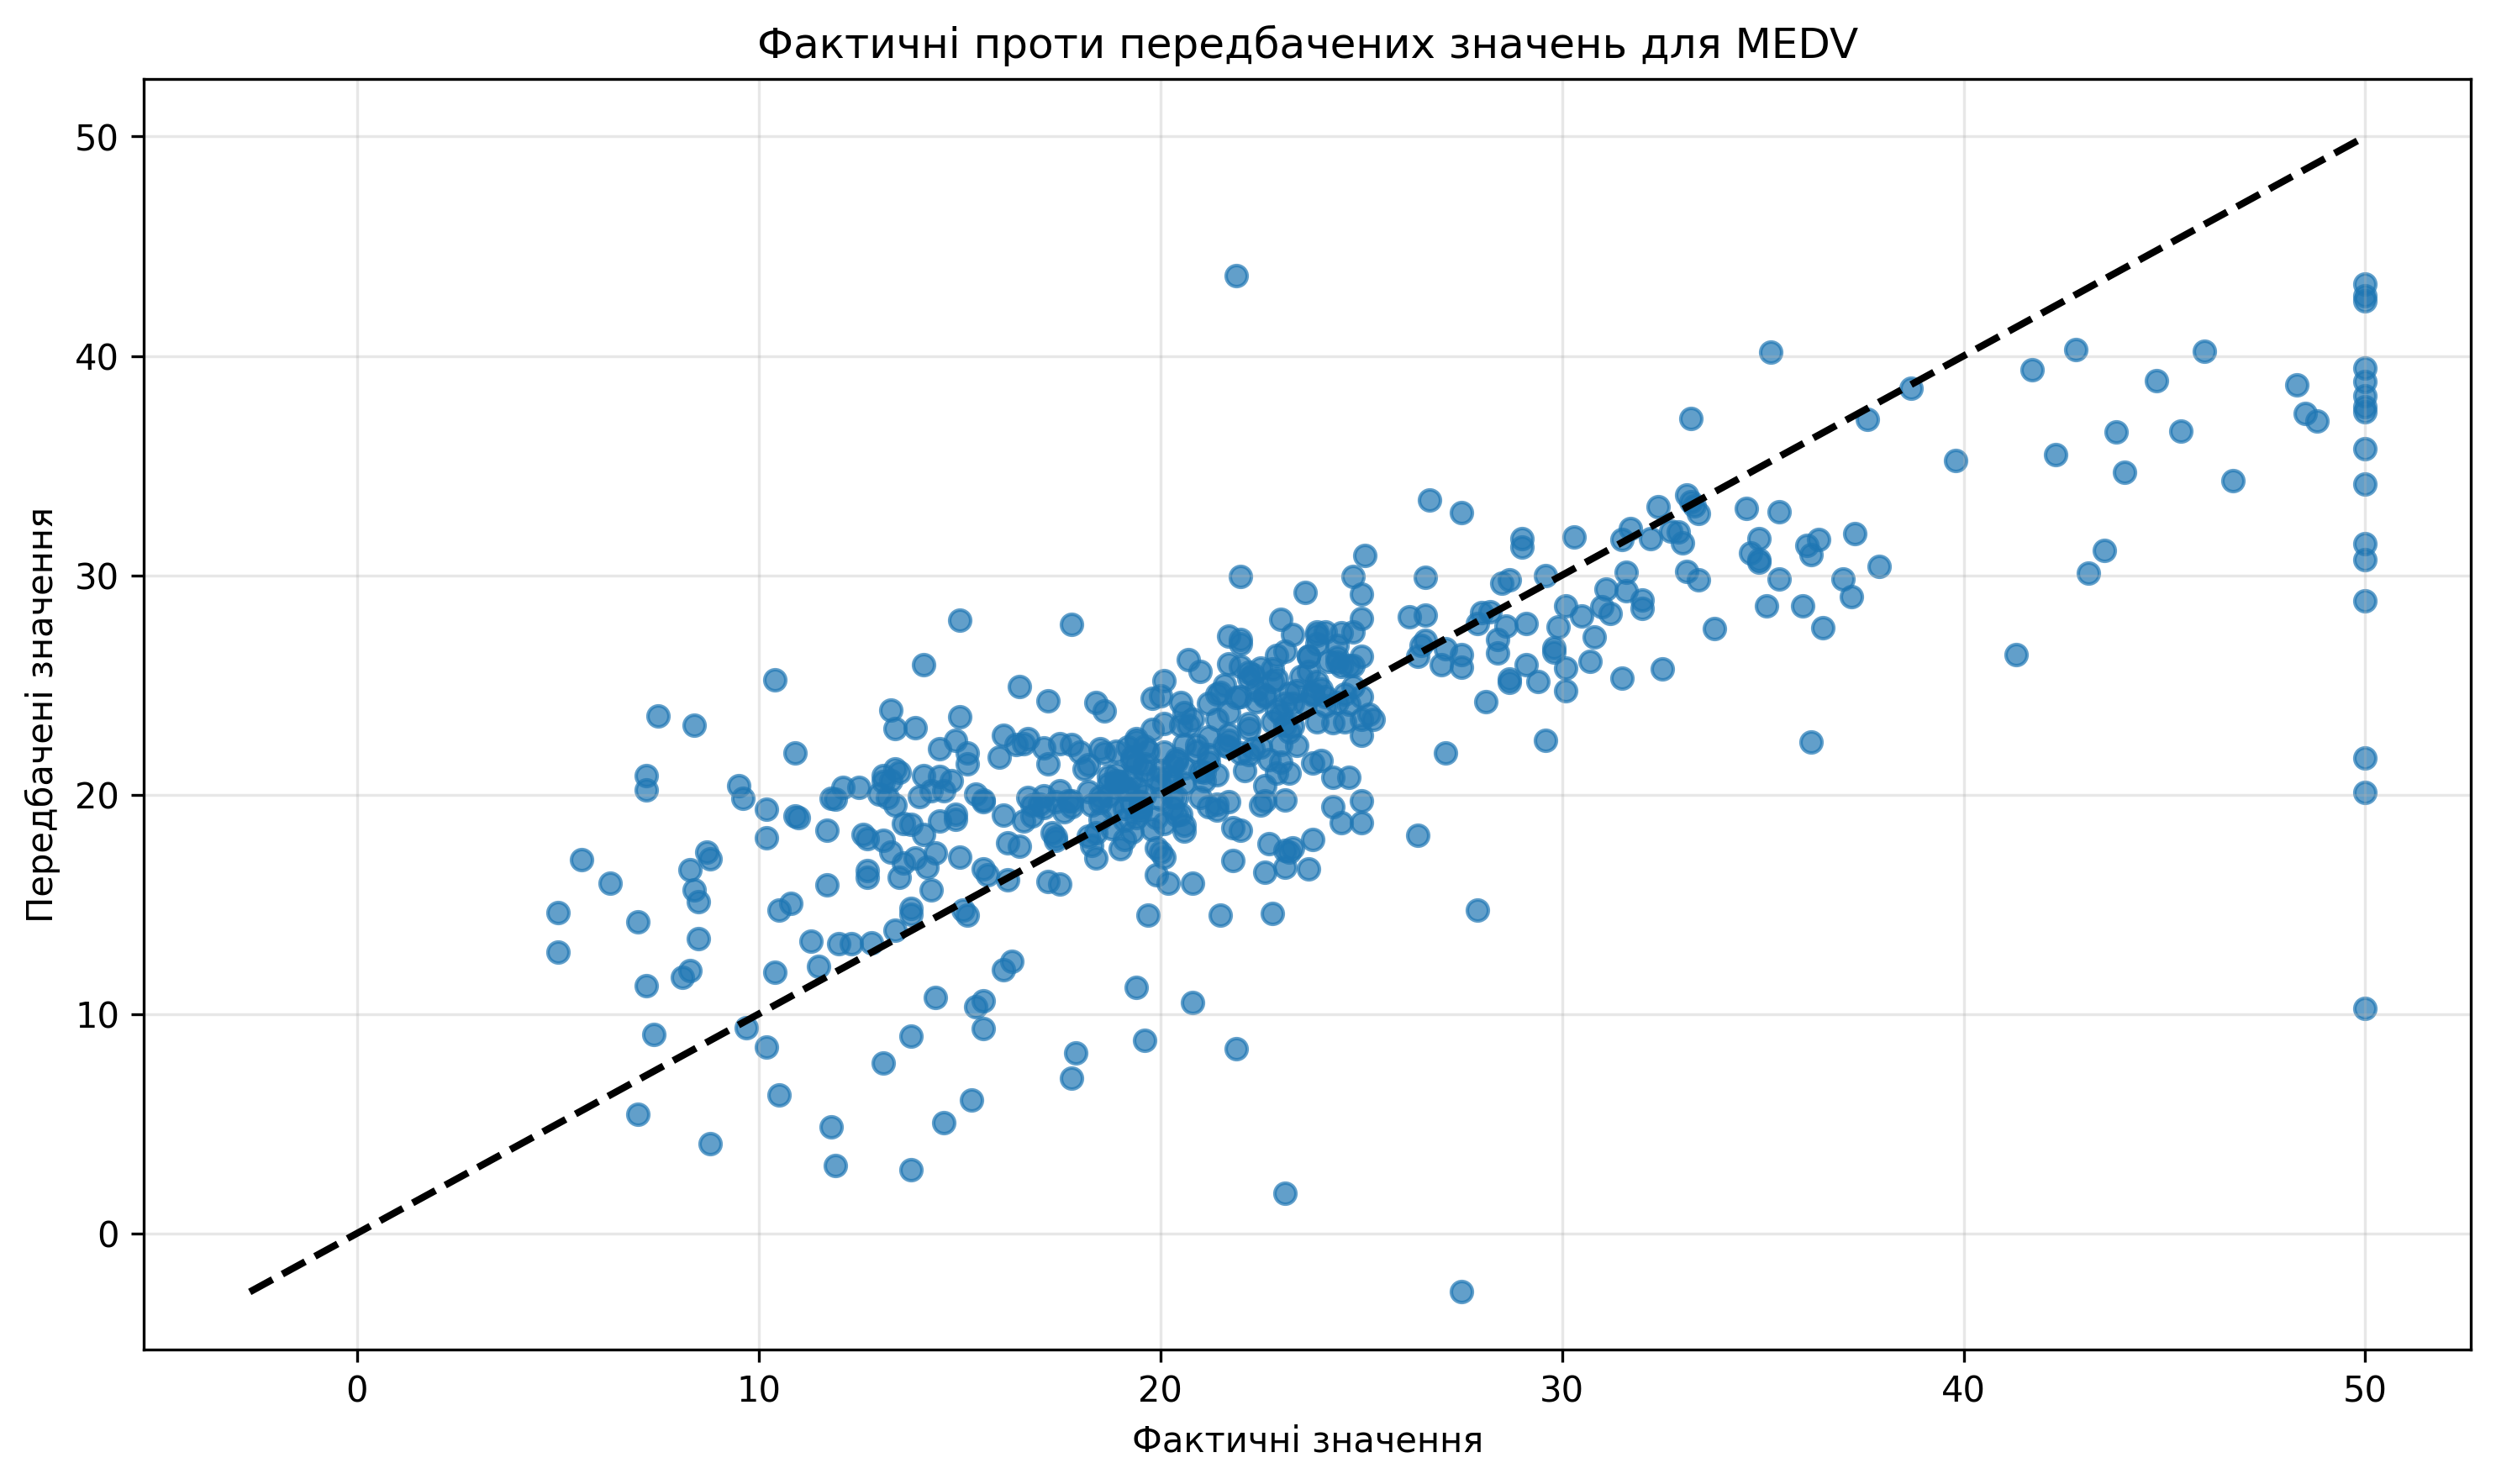
\includegraphics[width=0.8\textwidth]{actual_vs_predicted.png}
    \caption{Фактичні проти передбачених значень}
    \label{fig:фактичні_проти_передбачених_значень}
\end{figure}

\vspace{0.5cm}

\begin{figure}[H]
    \centering
    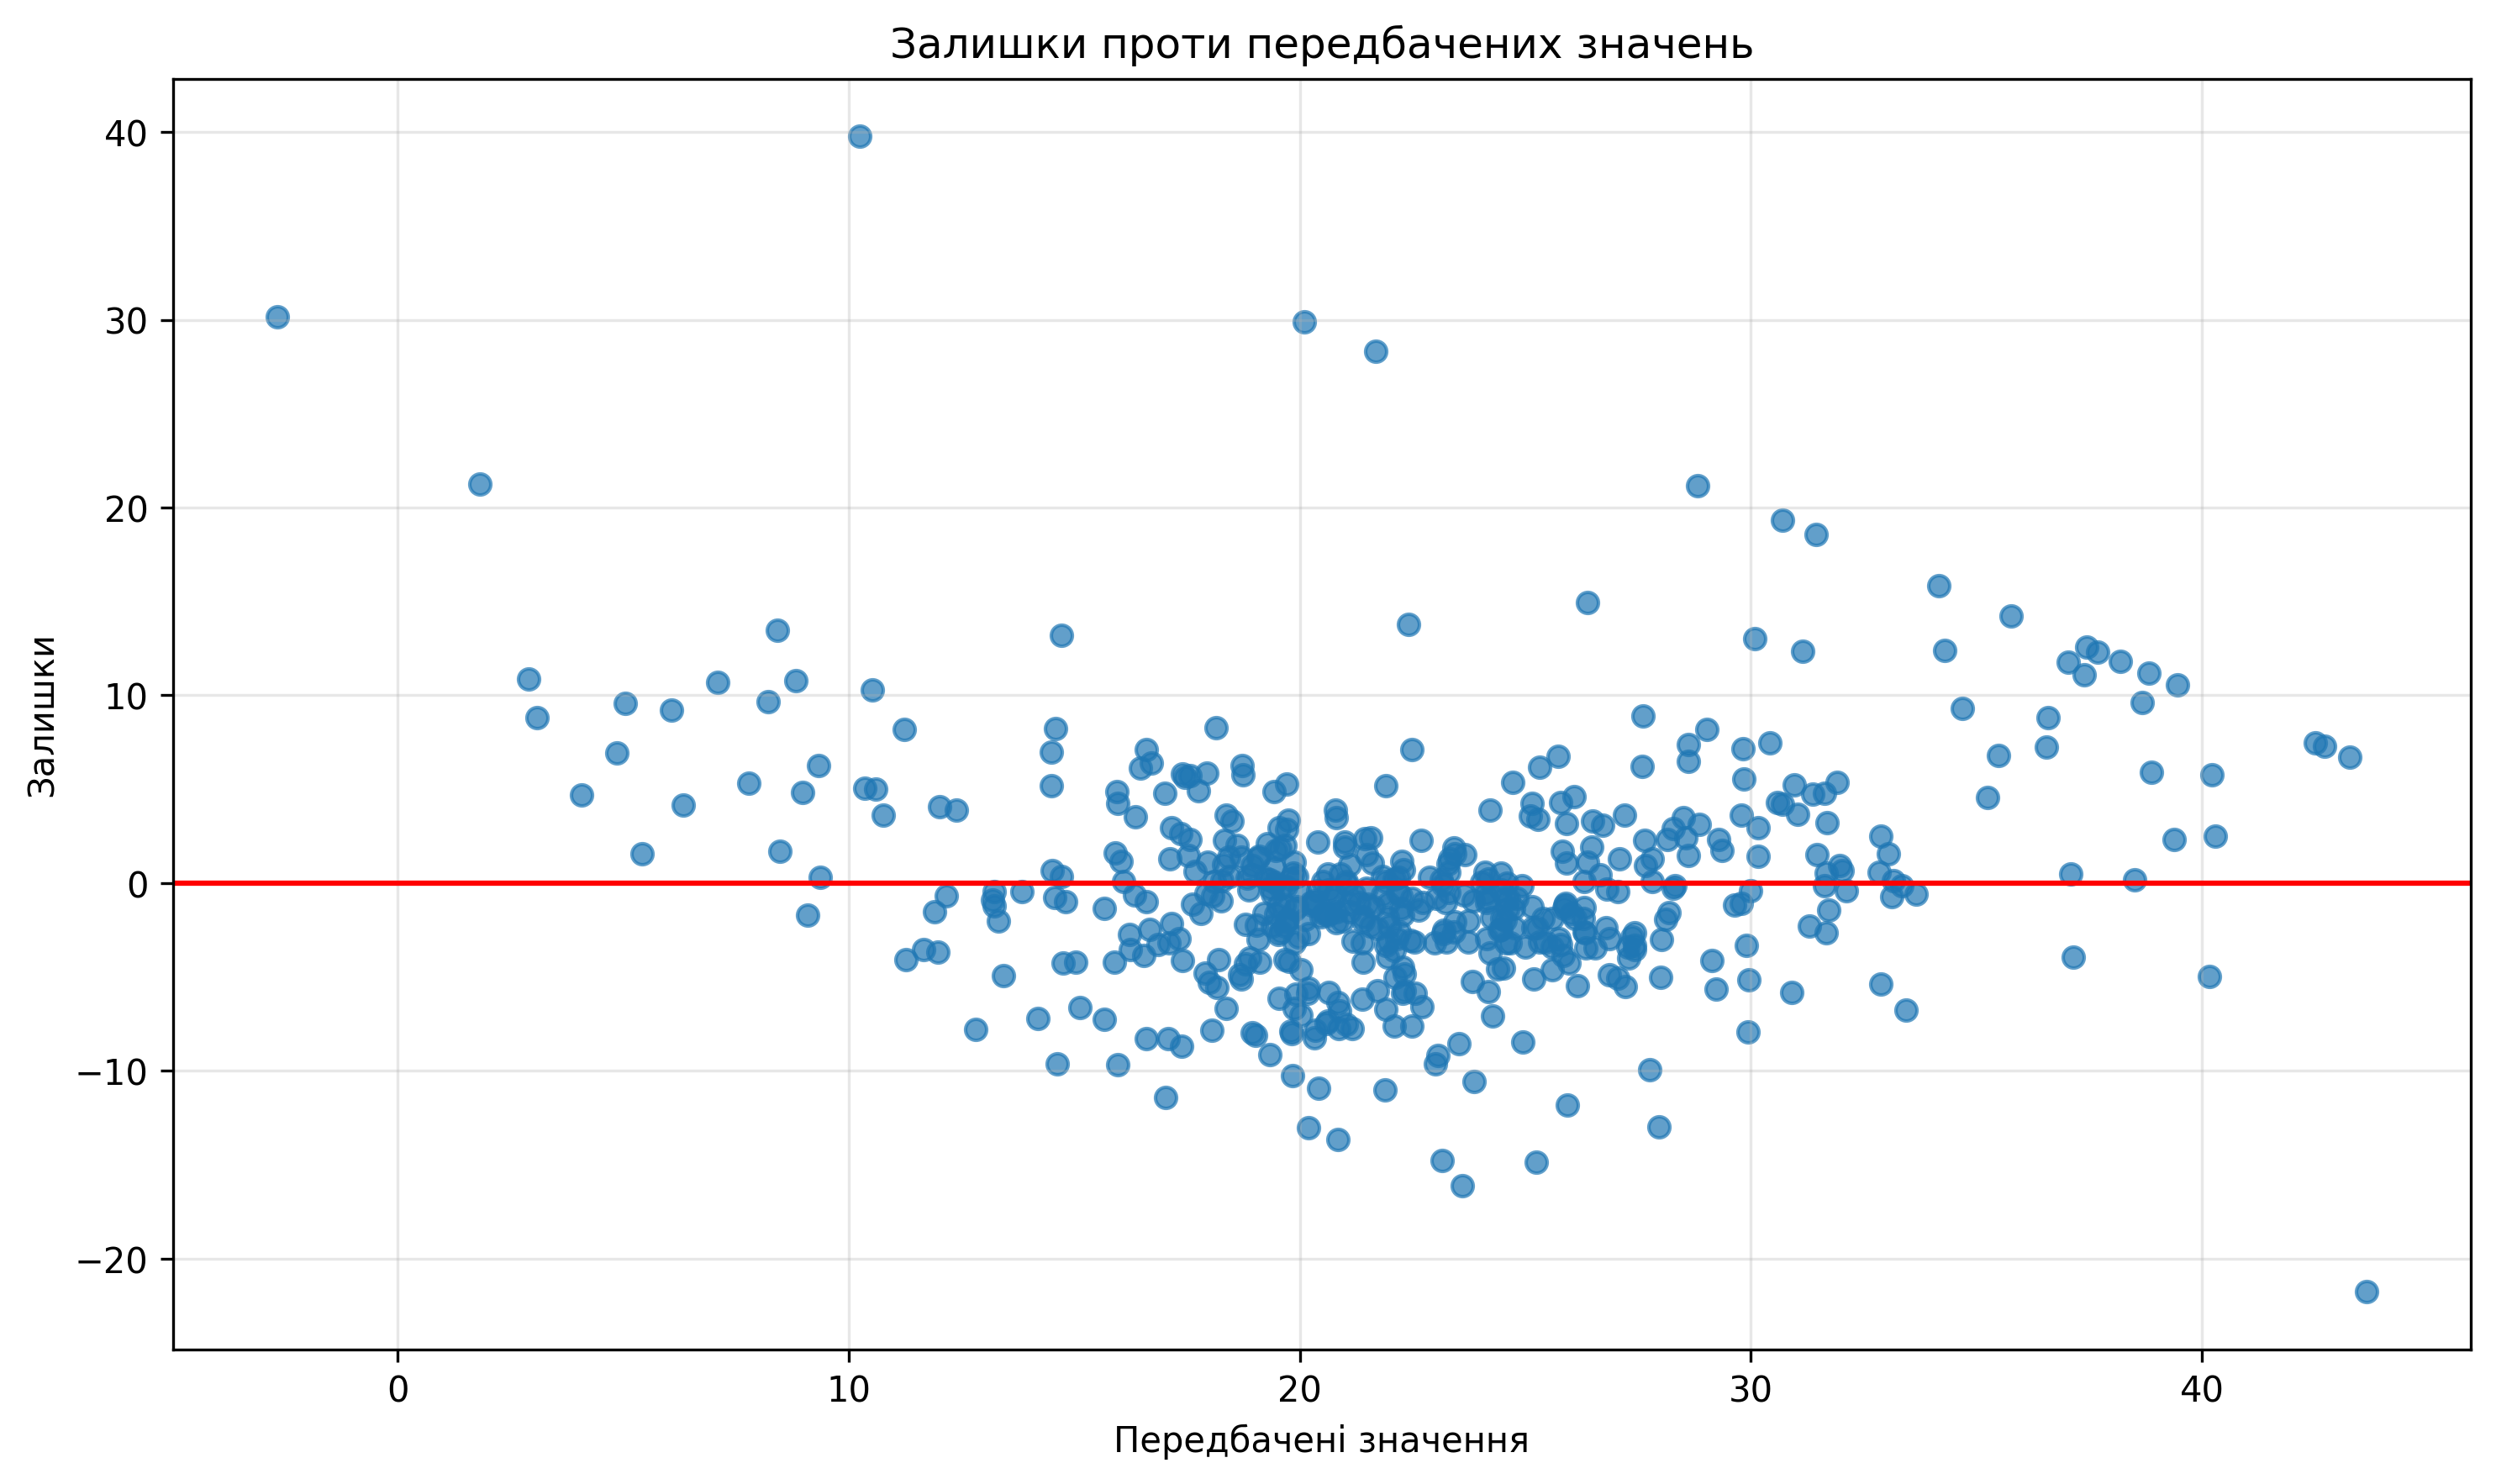
\includegraphics[width=0.8\textwidth]{residuals.png}
    \caption{Графік залишків}
    \label{fig:графік_залишків}
\end{figure}

\vspace{0.5cm}

\begin{figure}[H]
    \centering
    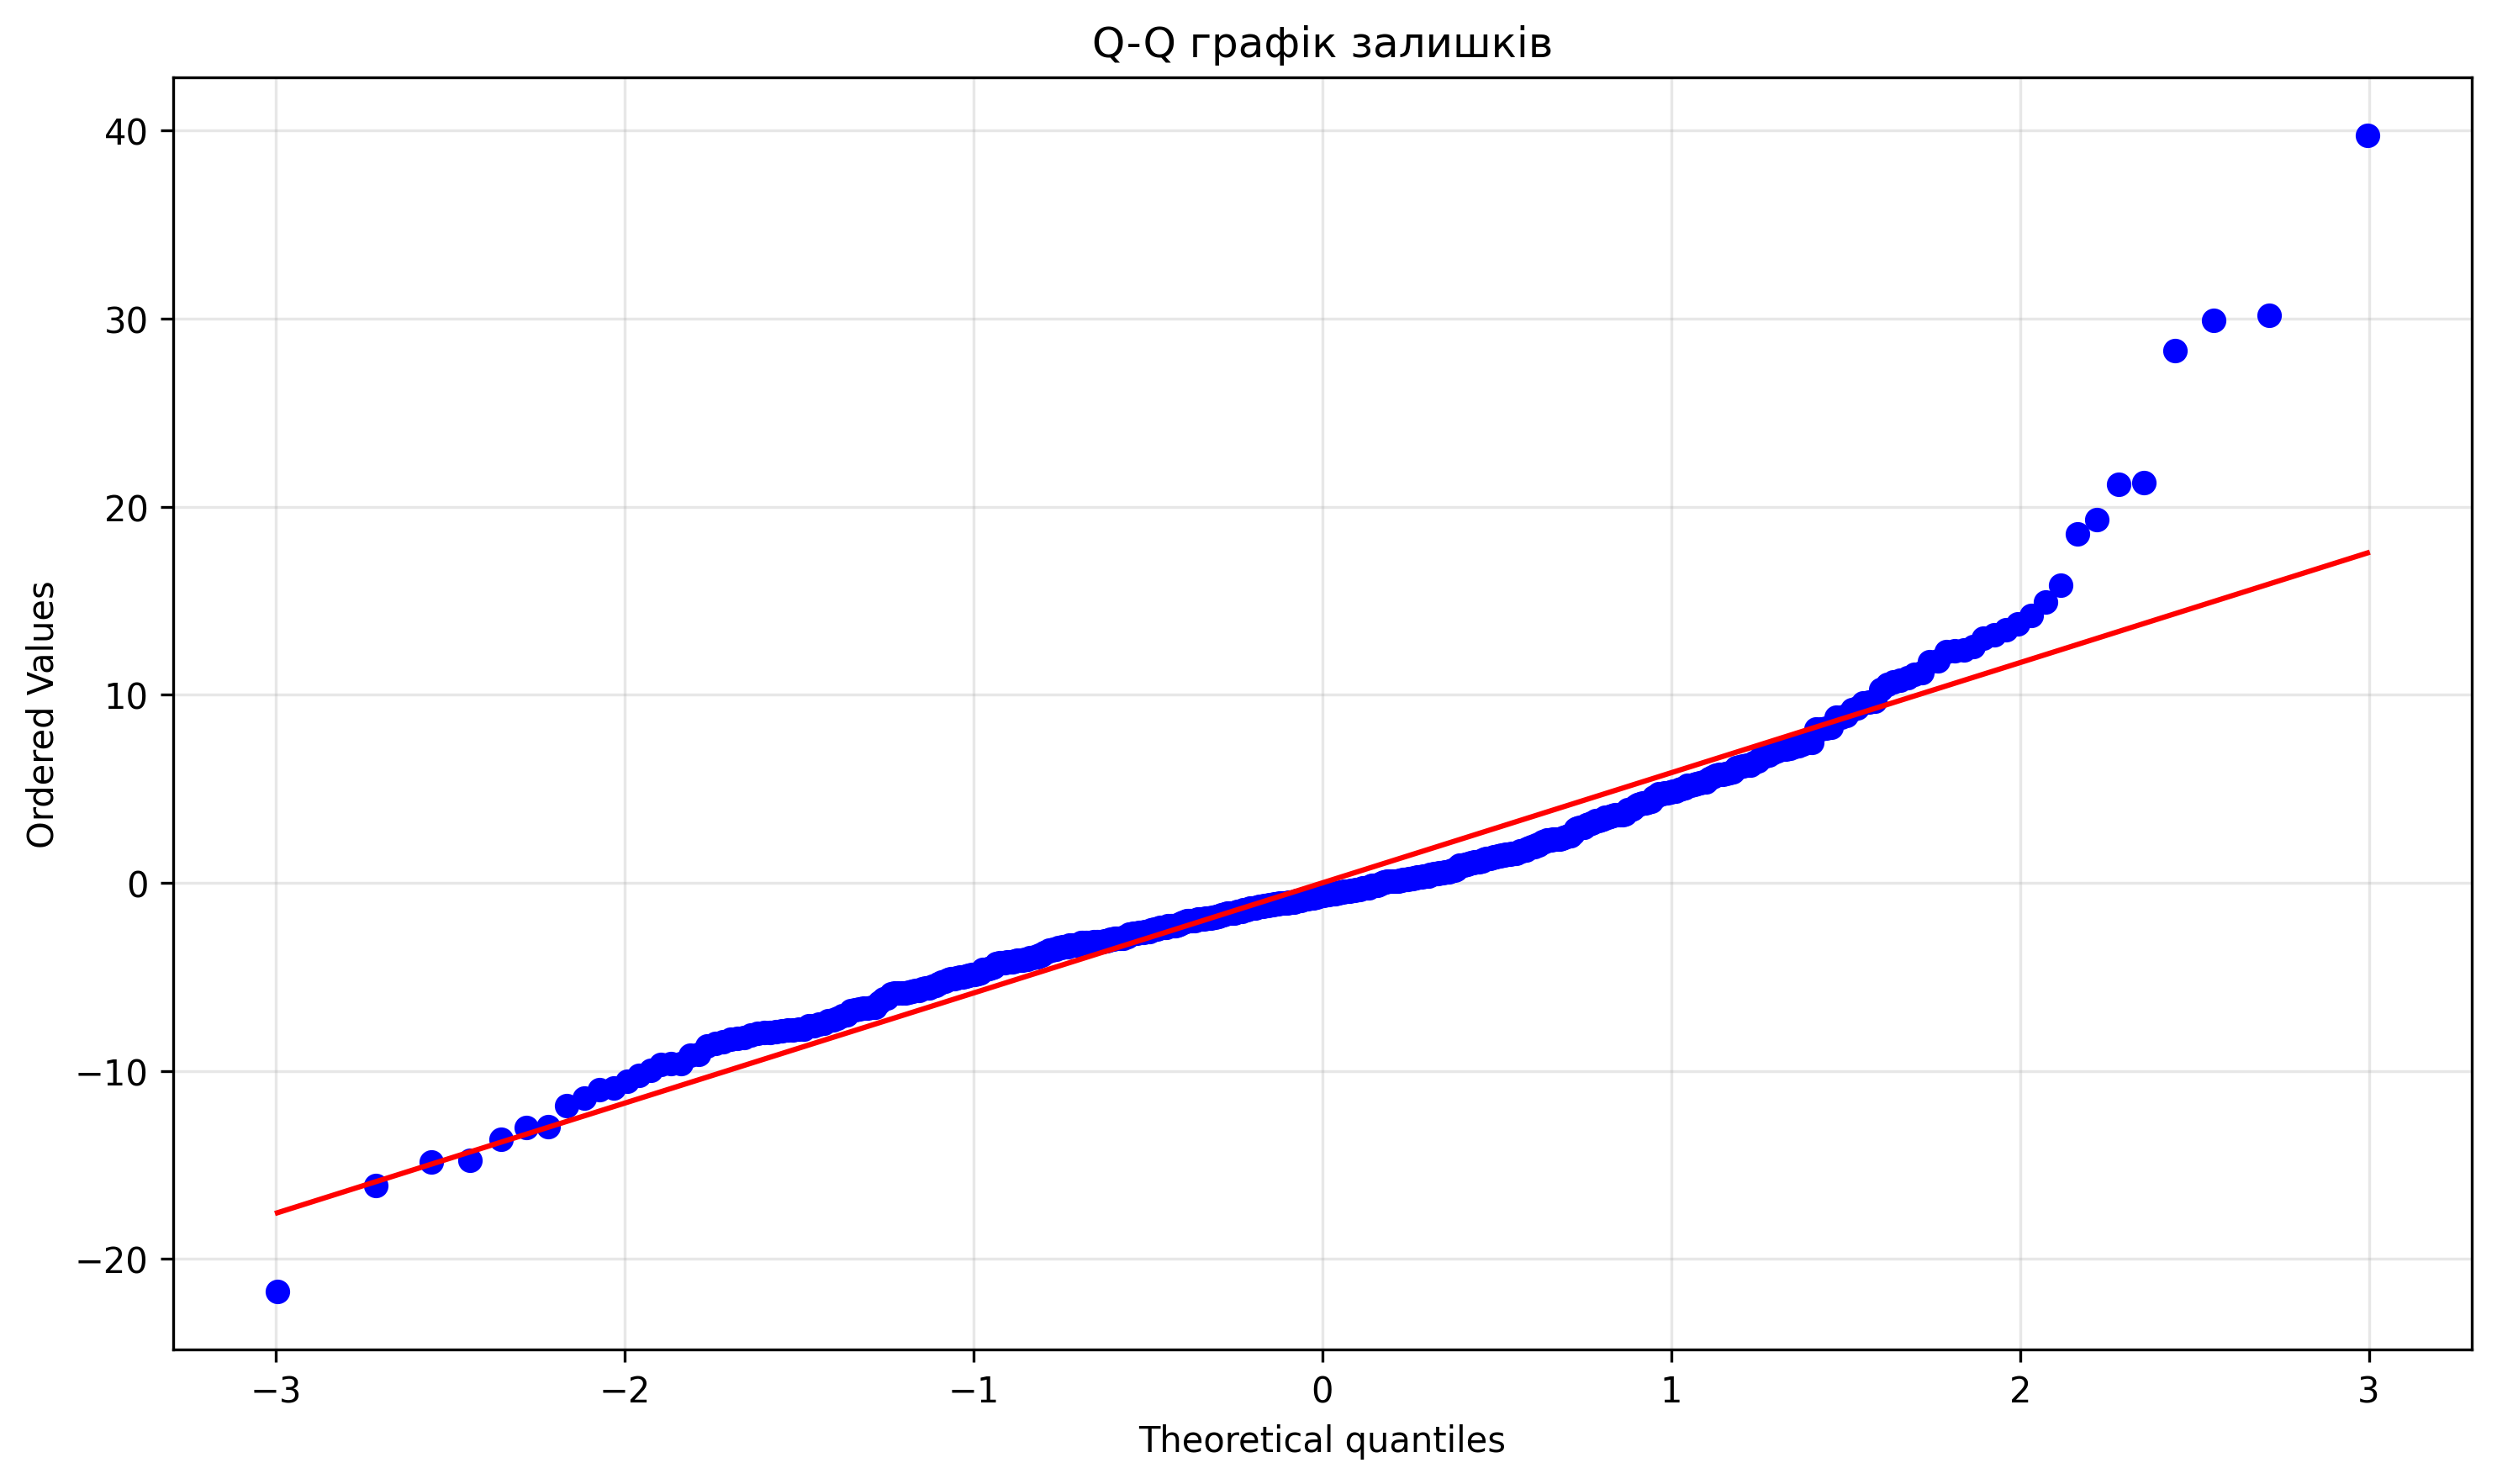
\includegraphics[width=0.8\textwidth]{qq_plot.png}
    \caption{Нормальний Q-Q графік залишків}
    \label{fig:нормальний_q-q_графік_залишків}
\end{figure}

\vspace{0.5cm}

\begin{figure}[H]
    \centering
    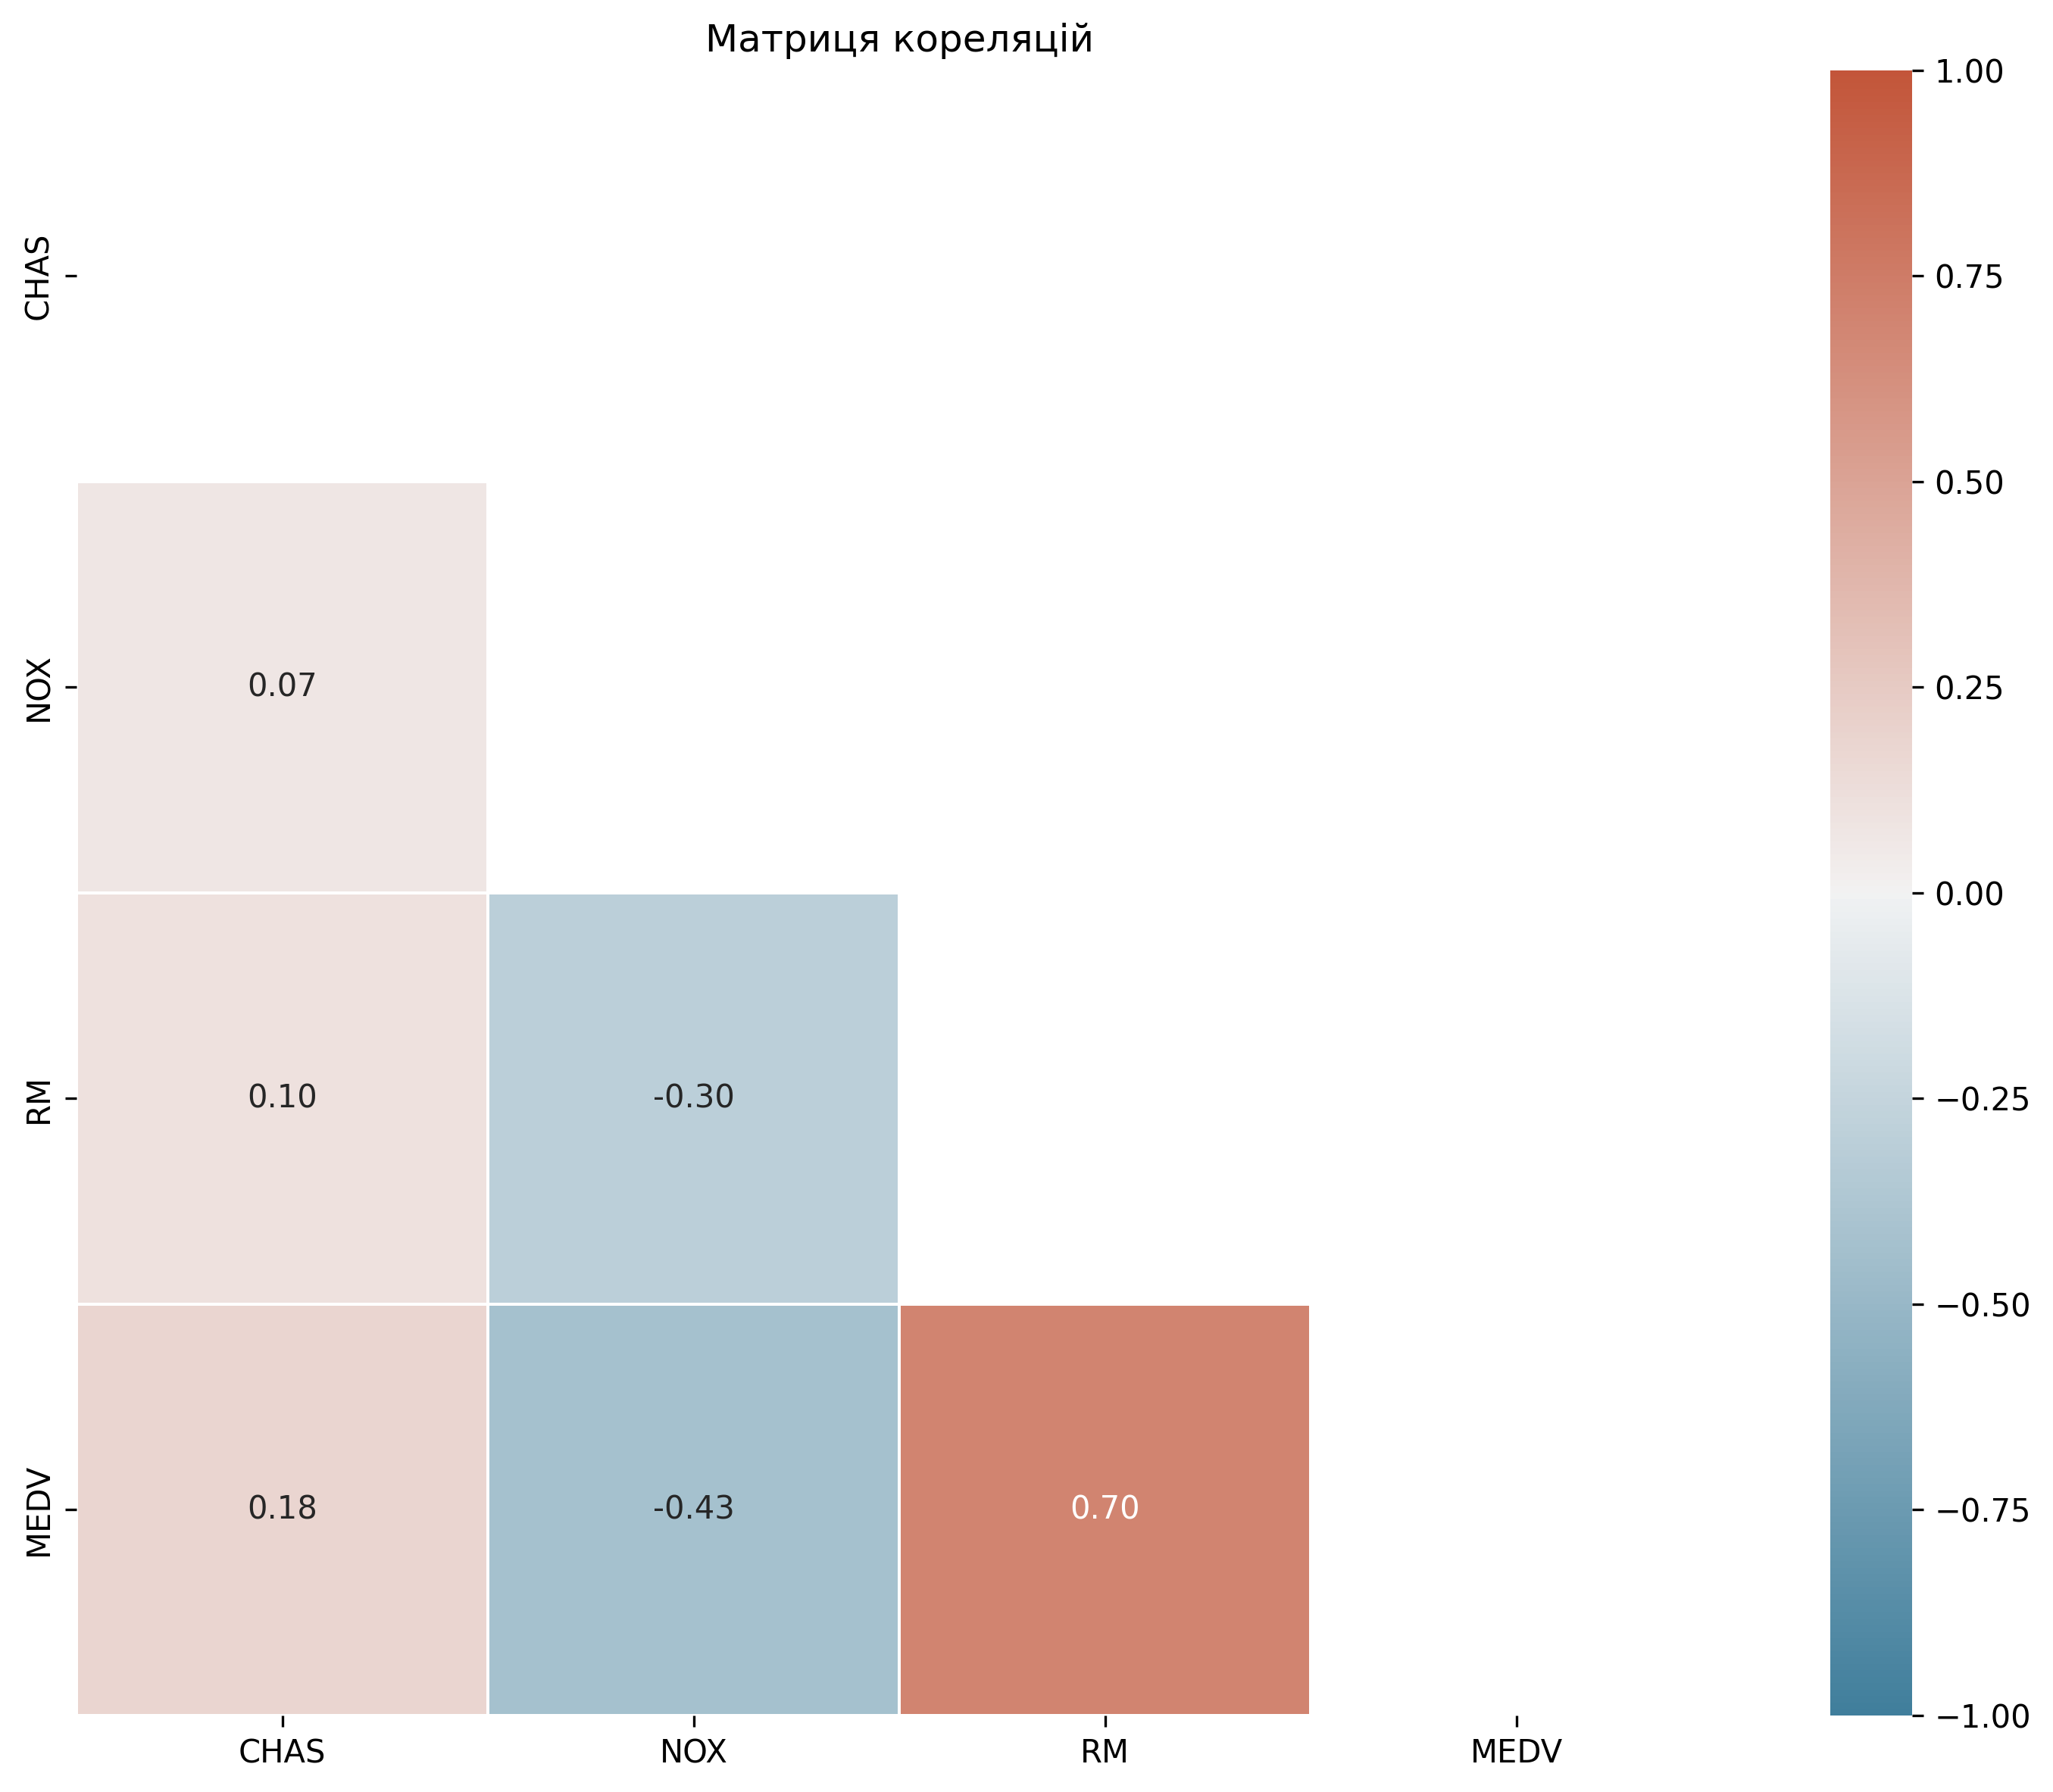
\includegraphics[width=0.8\textwidth]{correlation_heatmap.png}
    \caption{Теплова карта кореляцій}
    \label{fig:теплова_карта_кореляцій}
\end{figure}

\vspace{0.5cm}

\begin{figure}[H]
    \centering
    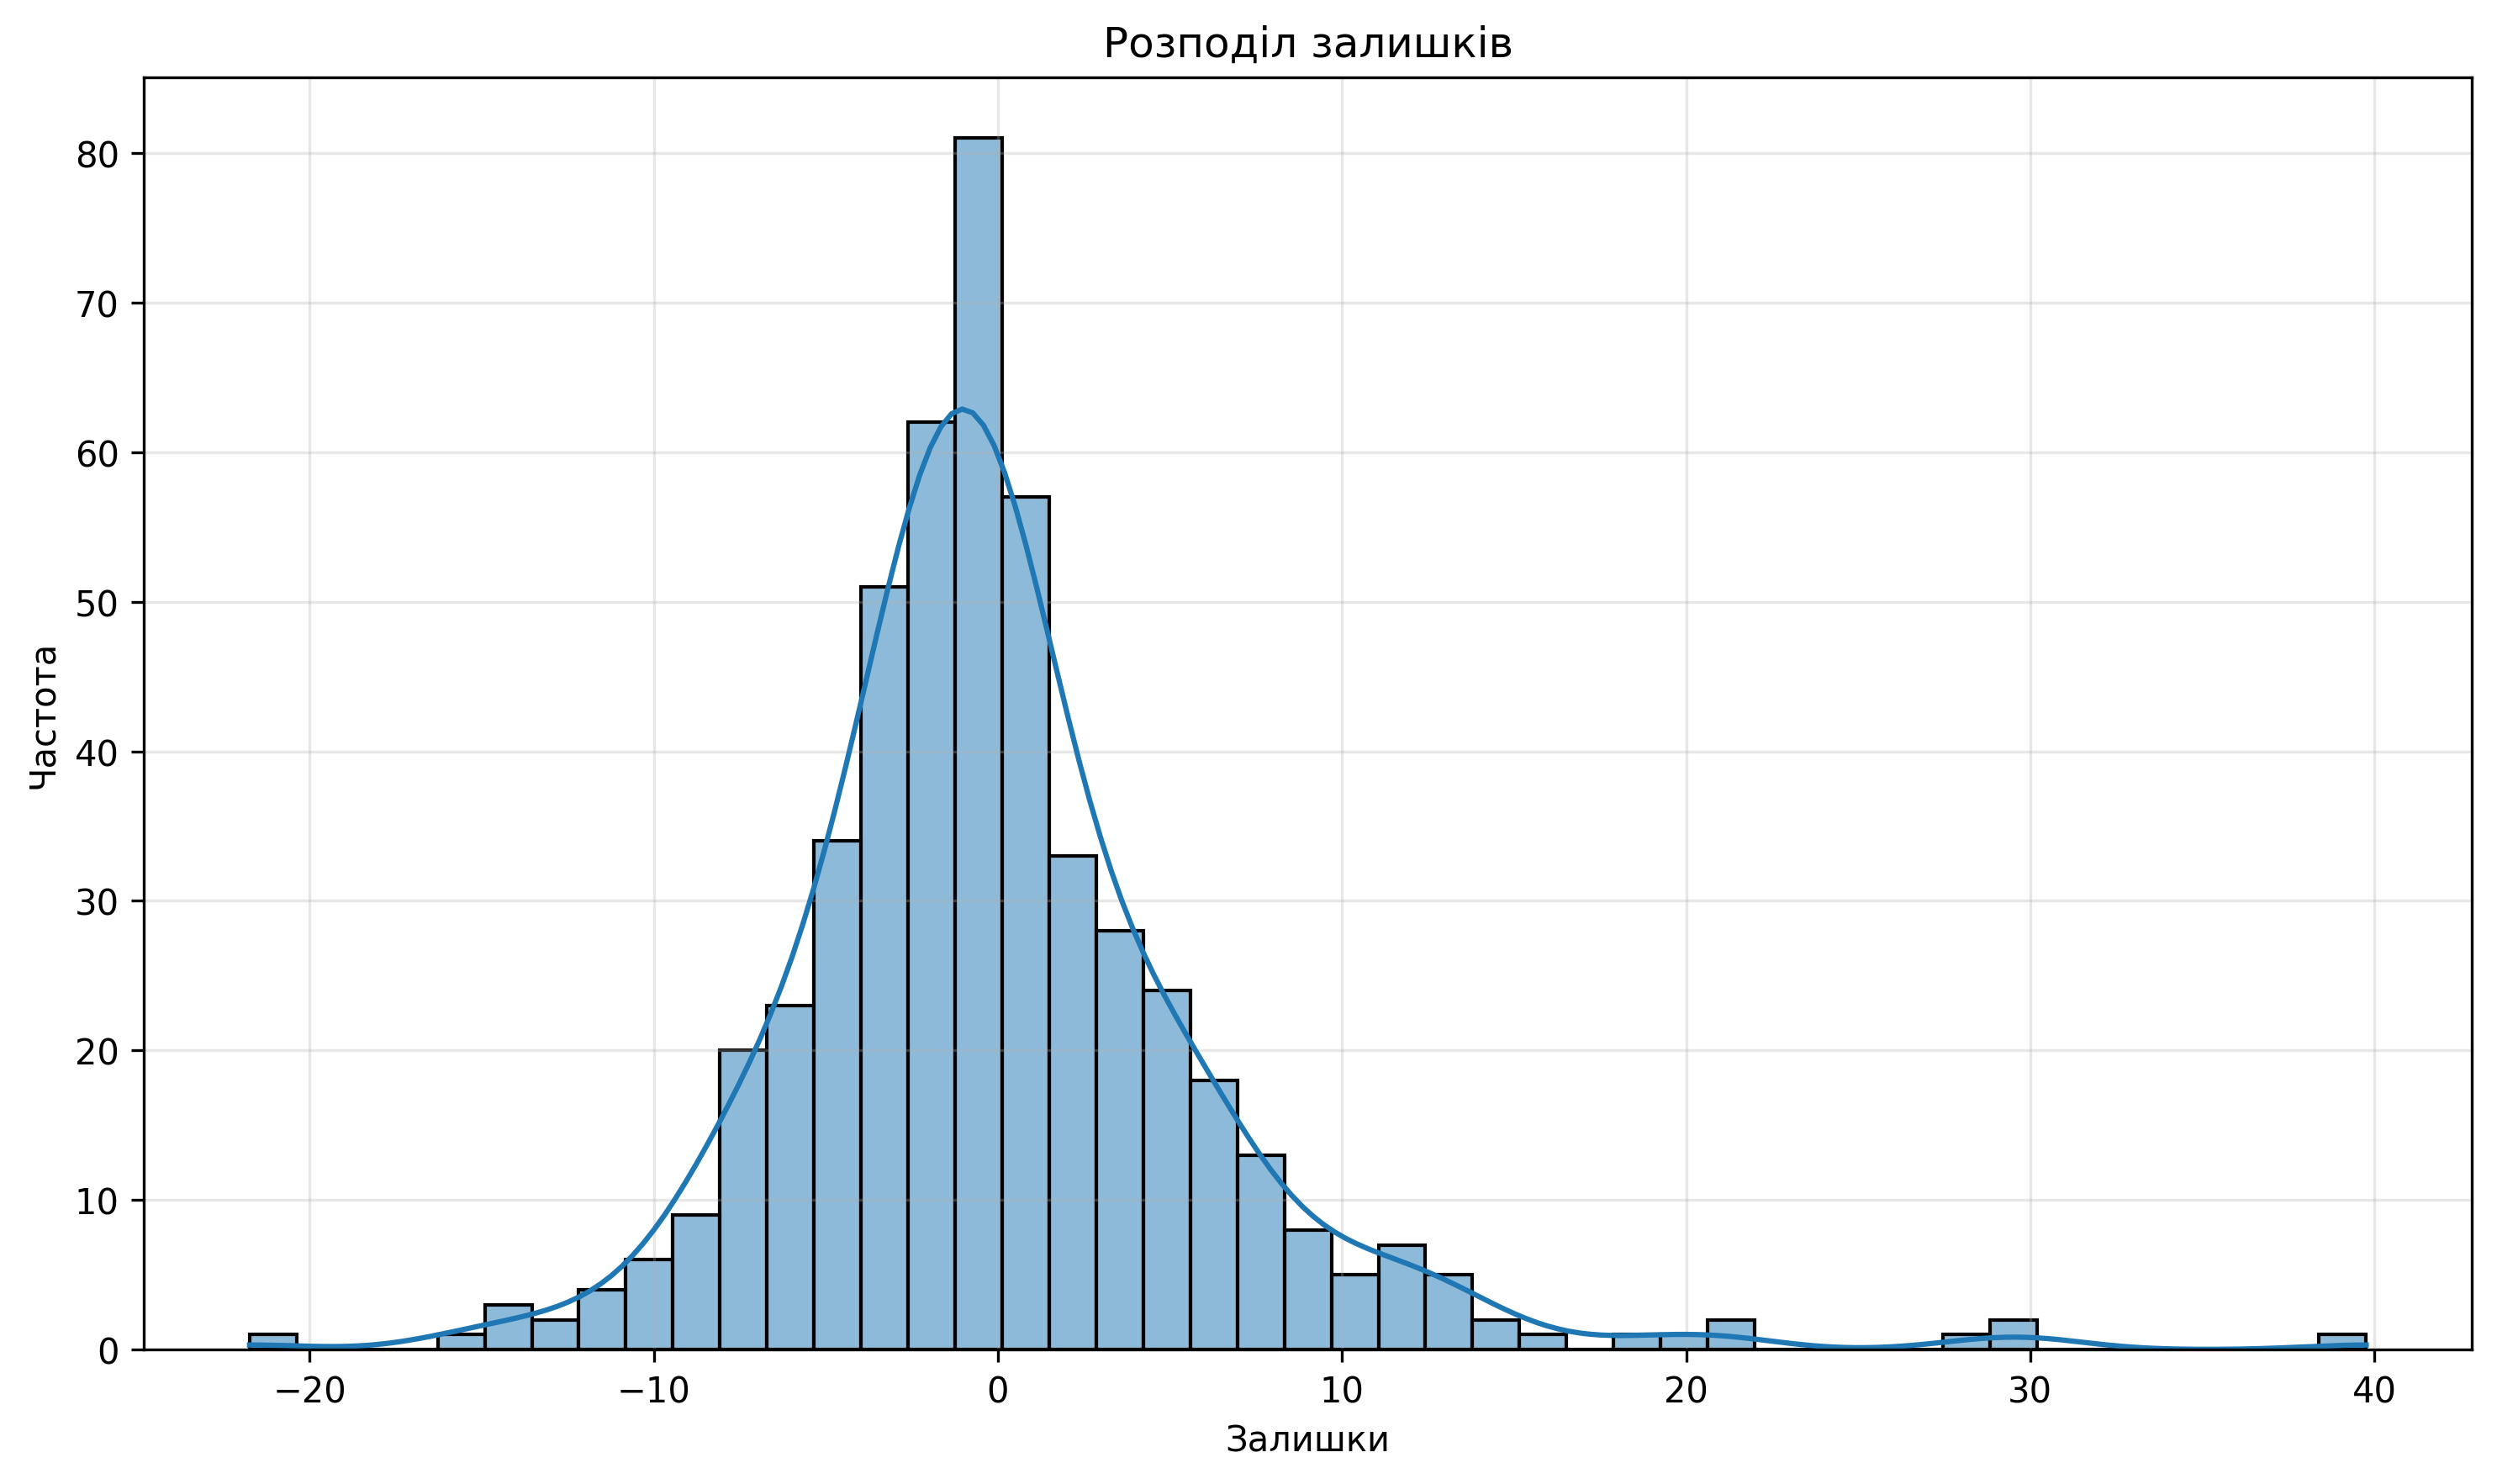
\includegraphics[width=0.8\textwidth]{residuals_hist.png}
    \caption{Гістограма залишків}
    \label{fig:гістограма_залишків}
\end{figure}

\vspace{0.5cm}

\section{Кореляційна матриця}

\begin{center}
\begin{tabular}{lcc}
\toprule
& Sample Question Papers Practiced & Sleep Hours \\
\midrule
Sample Question Papers Practiced & \textcolor{blue}{1.00} & 0.00 \\
Sleep Hours & 0.00 & \textcolor{blue}{1.00} \\

\bottomrule
\end{tabular}
\end{center}

\vspace{0.5cm}

\section{Інтерпретація результатів}

Дана модель багатофакторної лінійної регресії показує залежність змінної \textbf{Sleep Hours} від змінних \textbf{Sample Question Papers Practiced}.

Коефіцієнт детермінації $R^2$ дорівнює 0.0000, що означає, що 0.0\% варіації залежної змінної пояснюється включеними у модель незалежними змінними.

Середньоквадратична похибка (MSE) становить 2.8756, що є мірою середнього квадратичного відхилення спостережуваних значень від передбачених.

\vspace{0.5cm}

\section{Висновки}

Результати аналізу показують, що модель має низьку пояснювальну здатність.

Аналіз не виявив статистично значущих факторів (p < 0.05), що впливають на залежну змінну.

\end{document}
